\documentclass[12pt]{article}
\usepackage{amsmath}
\usepackage{amssymb}
\usepackage[letterpaper,margin=0.85in,centering]{geometry}
\usepackage{fancyhdr}
\usepackage{enumerate}
\usepackage{lastpage}
\usepackage{multicol}
\usepackage{graphicx}

\reversemarginpar

\pagestyle{fancy}
\cfoot{}
\lhead{Math 2560}\chead{Worksheet \# 4 Solutions}\rhead{Thursday 11\textsuperscript{th} February, 2016}
%\rfoot{Total: 10 points}
%\chead{{\bf Name:}}
\newcommand{\points}[1]{\marginpar{\hspace{24pt}[#1]}}
\newcommand{\skipline}{\vspace{12pt}}
%\renewcommand{\headrulewidth}{0in}
\headheight 30pt

\newcommand{\di}{\displaystyle}
\newcommand{\abs}[1]{\lvert #1\rvert}
\newcommand{\len}[1]{\lVert #1\rVert}
\renewcommand{\i}{\mathbf{i}}
\renewcommand{\j}{\mathbf{j}}
\renewcommand{\k}{\mathbf{k}}
\newcommand{\R}{\mathbb{R}}
\newcommand{\aaa}{\mathbf{a}}
\newcommand{\bbb}{\mathbf{b}}
\newcommand{\ccc}{\mathbf{c}}
\newcommand{\dotp}{\boldsymbol{\cdot}}
\newcommand{\bbm}{\begin{bmatrix}}
\newcommand{\ebm}{\end{bmatrix}}                   
                  
\begin{document}


%\author{Instructor: Sean Fitzpatrick}
\thispagestyle{fancy}
%\noindent{{\bf Name and student number:}}

\begin{enumerate}
 \item For each of the following sets of curves, sketch the curves to determine the area they enclose, and then find the area.
\begin{enumerate}
 \item $y=\sqrt{x+2}$, $y=\dfrac{1}{x+1}$, $x=0$ and $x=2$.

 \begin{center}
  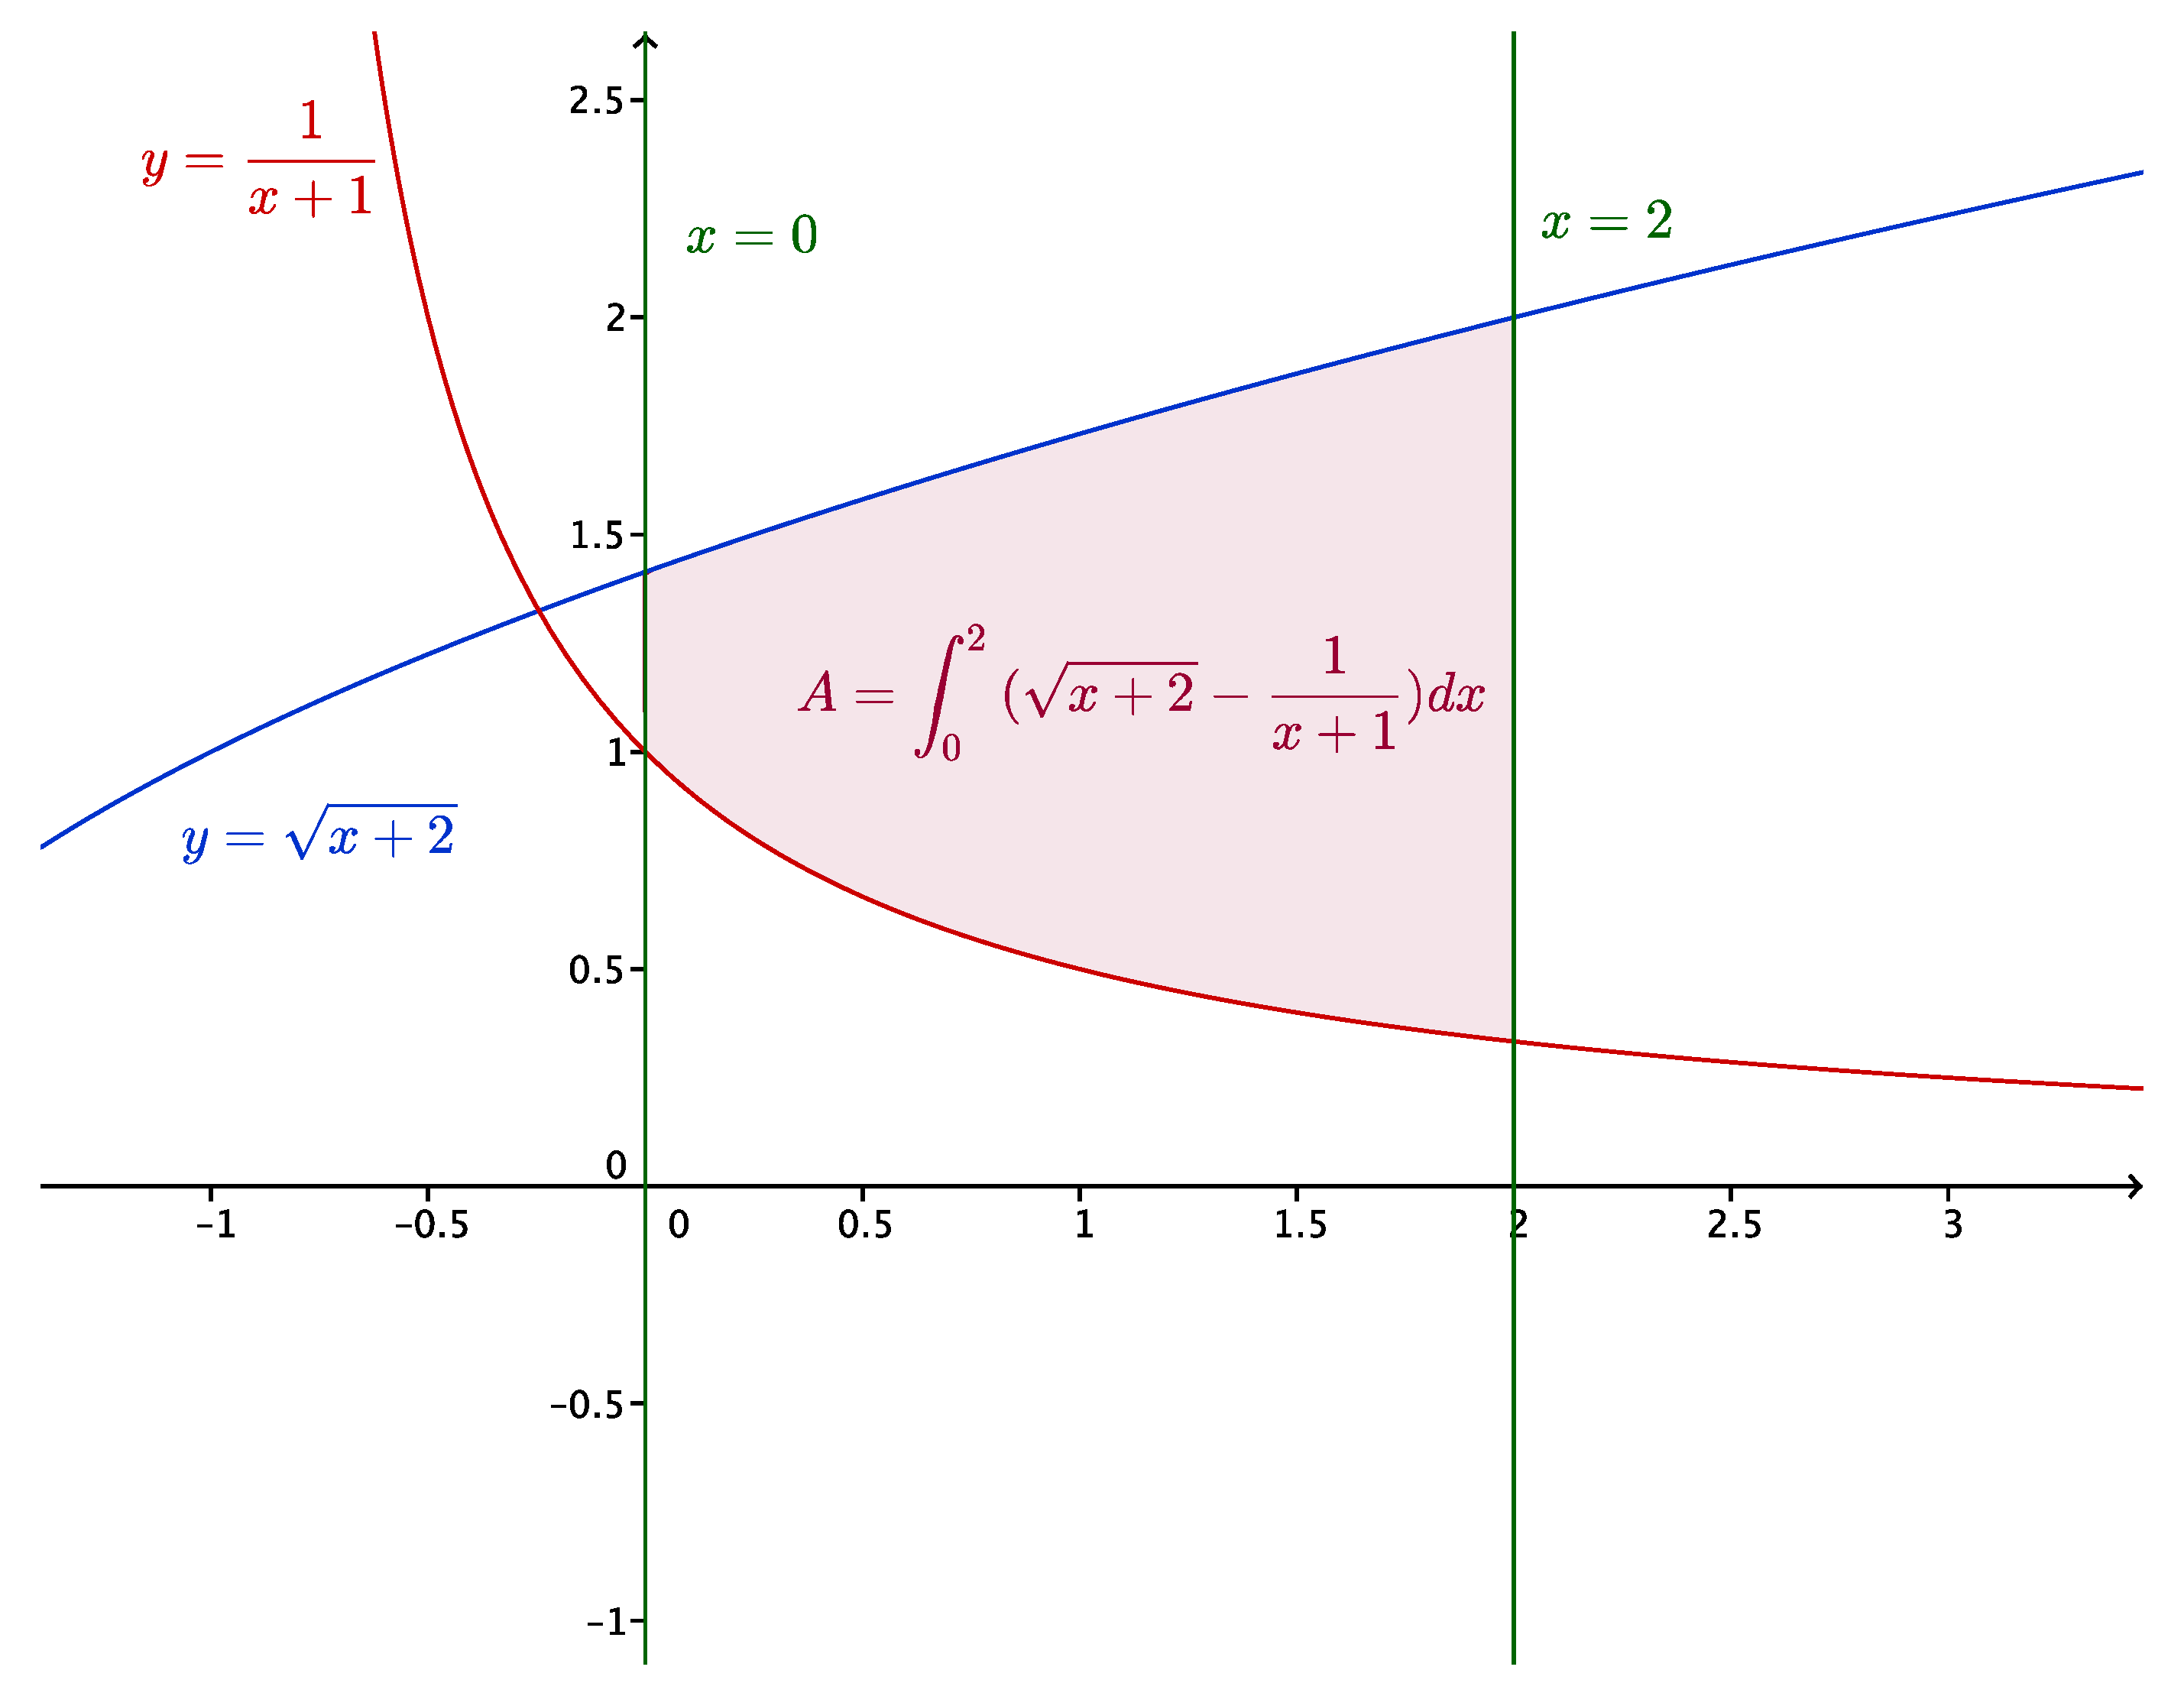
\includegraphics[width=0.8\textwidth]{WS4-1a}
 \end{center}
From the sketch we can see that $y=\sqrt{x+2}$ is the upper curve, and that there are no points of intersection between the given limits of integration. The area is therefore given by

\[
 A = \int_0^2\left((x+1)^{1/2}-\frac{1}{x+1}\right)\,dx = \left.\frac{2}{3}(x+2)^{3/2}-\ln(x+1)\right|_0^1 = \frac{16-4\sqrt{2}}{3}-\ln(3).
\]


\newpage

 \item $y=2x^2+5x-3$ and $y=x^2+4x-1$.
 \begin{center}
  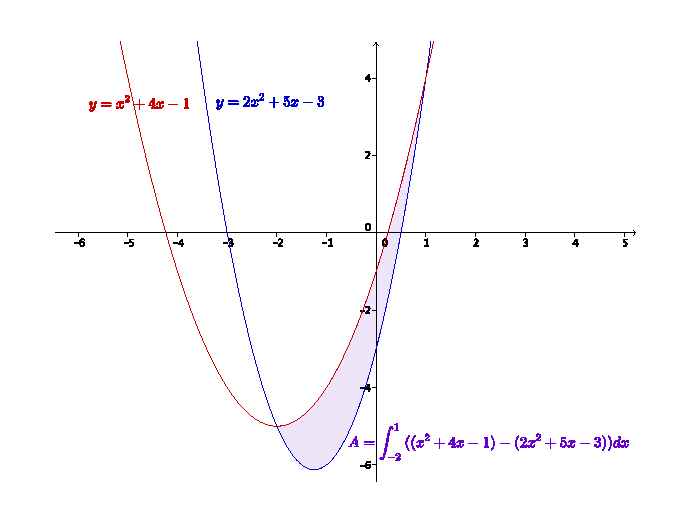
\includegraphics[width=0.8\textwidth]{WS4-1b}
 \end{center}
We see that the two curves intersect when $2x^2+5x-3=x^2+4x-1$, so $x^2+x-2=(x+2)(x-1)=0$, giving $x=-2, y=-5$ and $x=1, y=4$ as points of intersection. We also see that $(2x^2+5x-3)-(x^2+4x-1)=x^2+x-2<0$ for $-2<x<1$, giving us $y=x^2+4x-1$ as the upper curve. The area is therefore

\[
 A = \int_{-2}^1[(x^2+4x-1)-(2x^2+5x-2)]\,dx = \int_{-2}^1(2-x-x^2)\,dx = \left. 2x-\frac{x^2}{2}-\frac{x^3}{3}\right|_{-2}^1 = \frac{9}{2}.
\]

\newpage

 \item $y=x^2+1$, $y=\frac{1}{4}(x-3)^2+1$, and $y=1$.

\begin{center}
 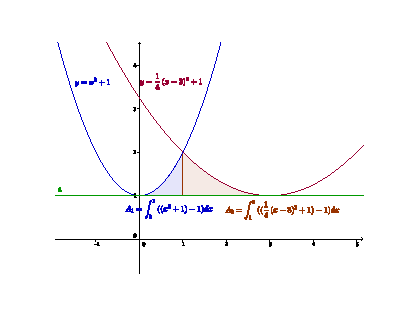
\includegraphics[width=0.8\textwidth]{WS4-1c}
\end{center}

In this case, when we plot the curves, we see that there are two regions of integration to consider. First, we note that the curves $y=x^2+1$ and $y=\frac{1}{4}(x-3)^2+1$ intersect when $x^2+1=\frac{1}{4}(x-3)^2+1$, so $x^2=\frac{1}{4}(x-3)^2$, which gives $4x^2=x^2-6x+9$, and thus $3x^2+6x-9=3(x+3)(x-1)=0$. The intersection of the two curves in the first quadrant thus occurs when $x=1, y=2$. The desired area is therefore the area below $y=x^2+1$ and above $y=1$ for $0\leq x\leq 1$ and below $y=\frac{1}{4}(x-3)^2+1$ and above $y=1$ for $1\leq x\leq 3$. This gives us
\begin{align*}
 A & = \int_0^1[(x^2+1)-1]\,dx+\int_1^3[(\frac{1}{4}(x-3)^2+1)-1]\,dx\\
& = \left.\left(\frac{x^3}{3}\right)\right|_0^1 + \left.\left(\frac{1}{12}(x-3)^3\right)\right|_1^3\\
& = \frac{1}{3}-0+0-\frac{1}{12}(-2)^3 = 1.
\end{align*}

\newpage

 \item $y=\cos x$ and $y=\sin 2x$, between $x=0$ and $x=\pi/2$.

\begin{center}
 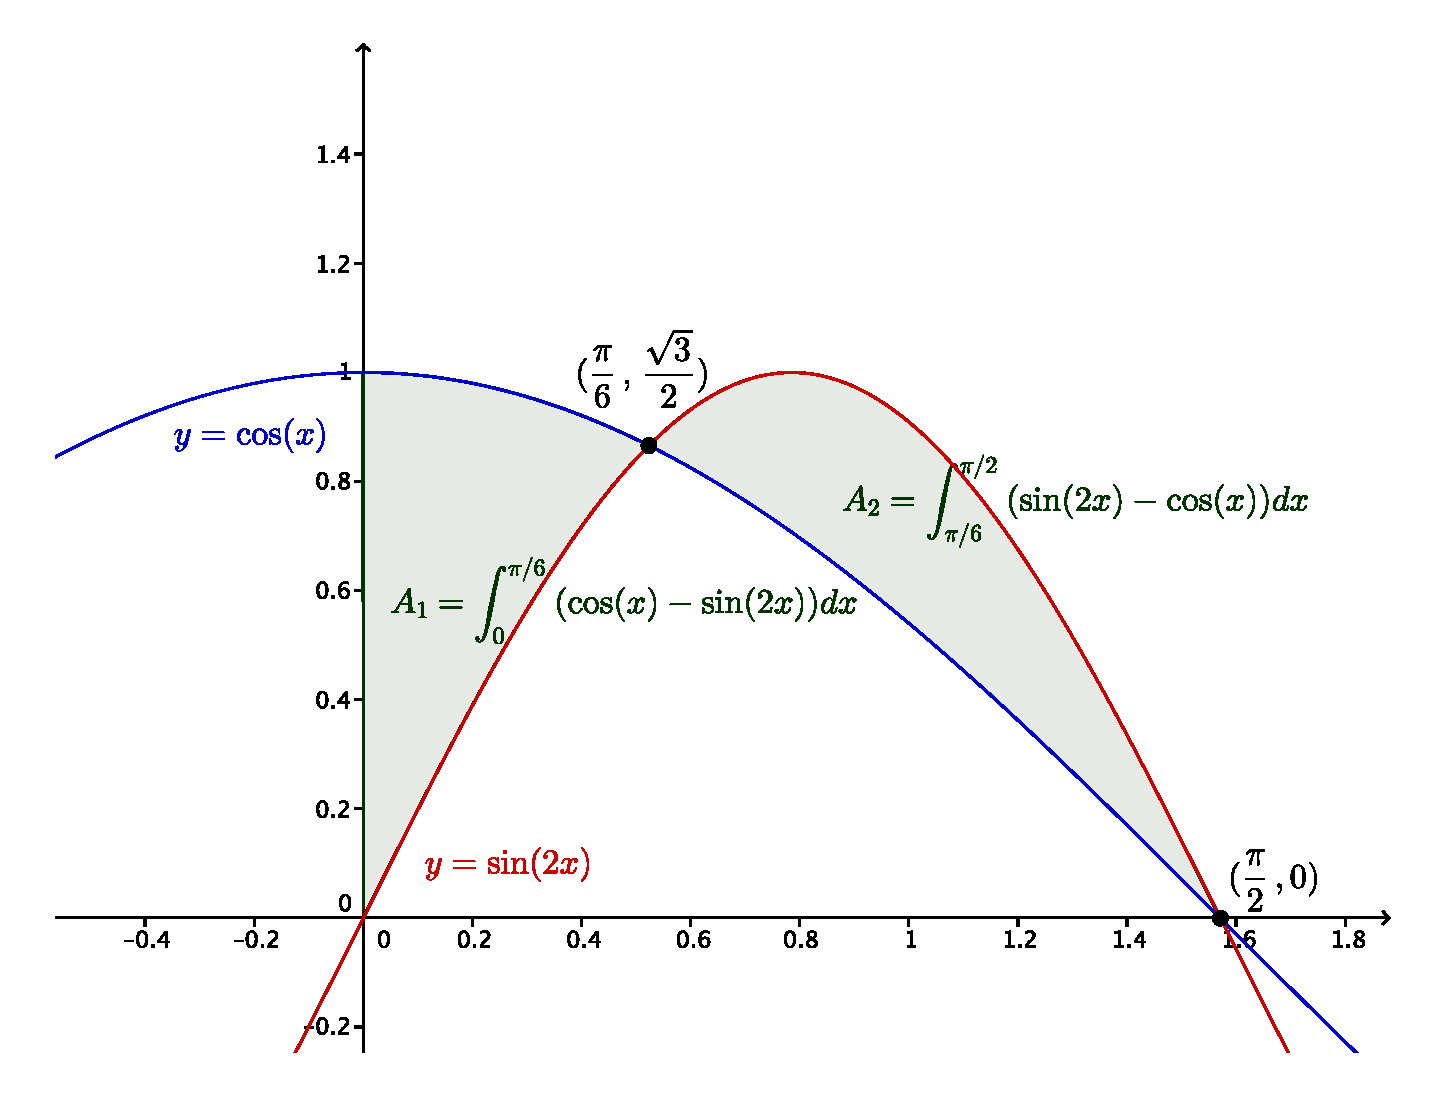
\includegraphics[width=0.8\textwidth]{WS4-1d}
\end{center}

From the sketch above, we see that the two curves change position once between $0$ and $\frac{\pi}{2}$, so we need to find the point of intersection. If $\cos x = \sin(2x) = 2\sin(x)\cos(x)$, we get $\cos(x)(2\sin(x)-1)=0$, so either $\cos(x)=0$ or $2\sin(x)=1$. On the interval $[0,\frac{\pi}{2}]$ we only have $\cos(x)=0$ when $x=\frac{\pi}{2}$, while $\sin(x)=\frac{1}{2}$ for $x=\frac{\pi}{6}$. The point of intersection is therefore at $x=\frac{\pi}{6}$, $y=\frac{\sqrt{3}}{2}$. The area is given by
\begin{align*}
 A & = \int_0^{\pi/6}(\cos (x) -\sin (2x))\,dx + \int_{\pi/6}^{\pi/2}(\sin(2x)-\cos(x))\,dx\\
& = \left.(\sin x+\frac{1}{2}\cos(2x))\right|_0^{\pi/6} + \left.(-\frac{1}{2}\cos(2x)-\sin(x))\right|_{\pi/6}^{\pi/2}\\
& = \frac{1}{2}+\frac{1}{4}-0-\frac{1}{2}-\frac{1}{2}(-1)-1+\frac{1}{4}+\frac{1}{2}\\
& = \frac{1}{2}.
\end{align*}
\newpage

 \item $y=x$ and $y=x^3$.

\begin{center}
 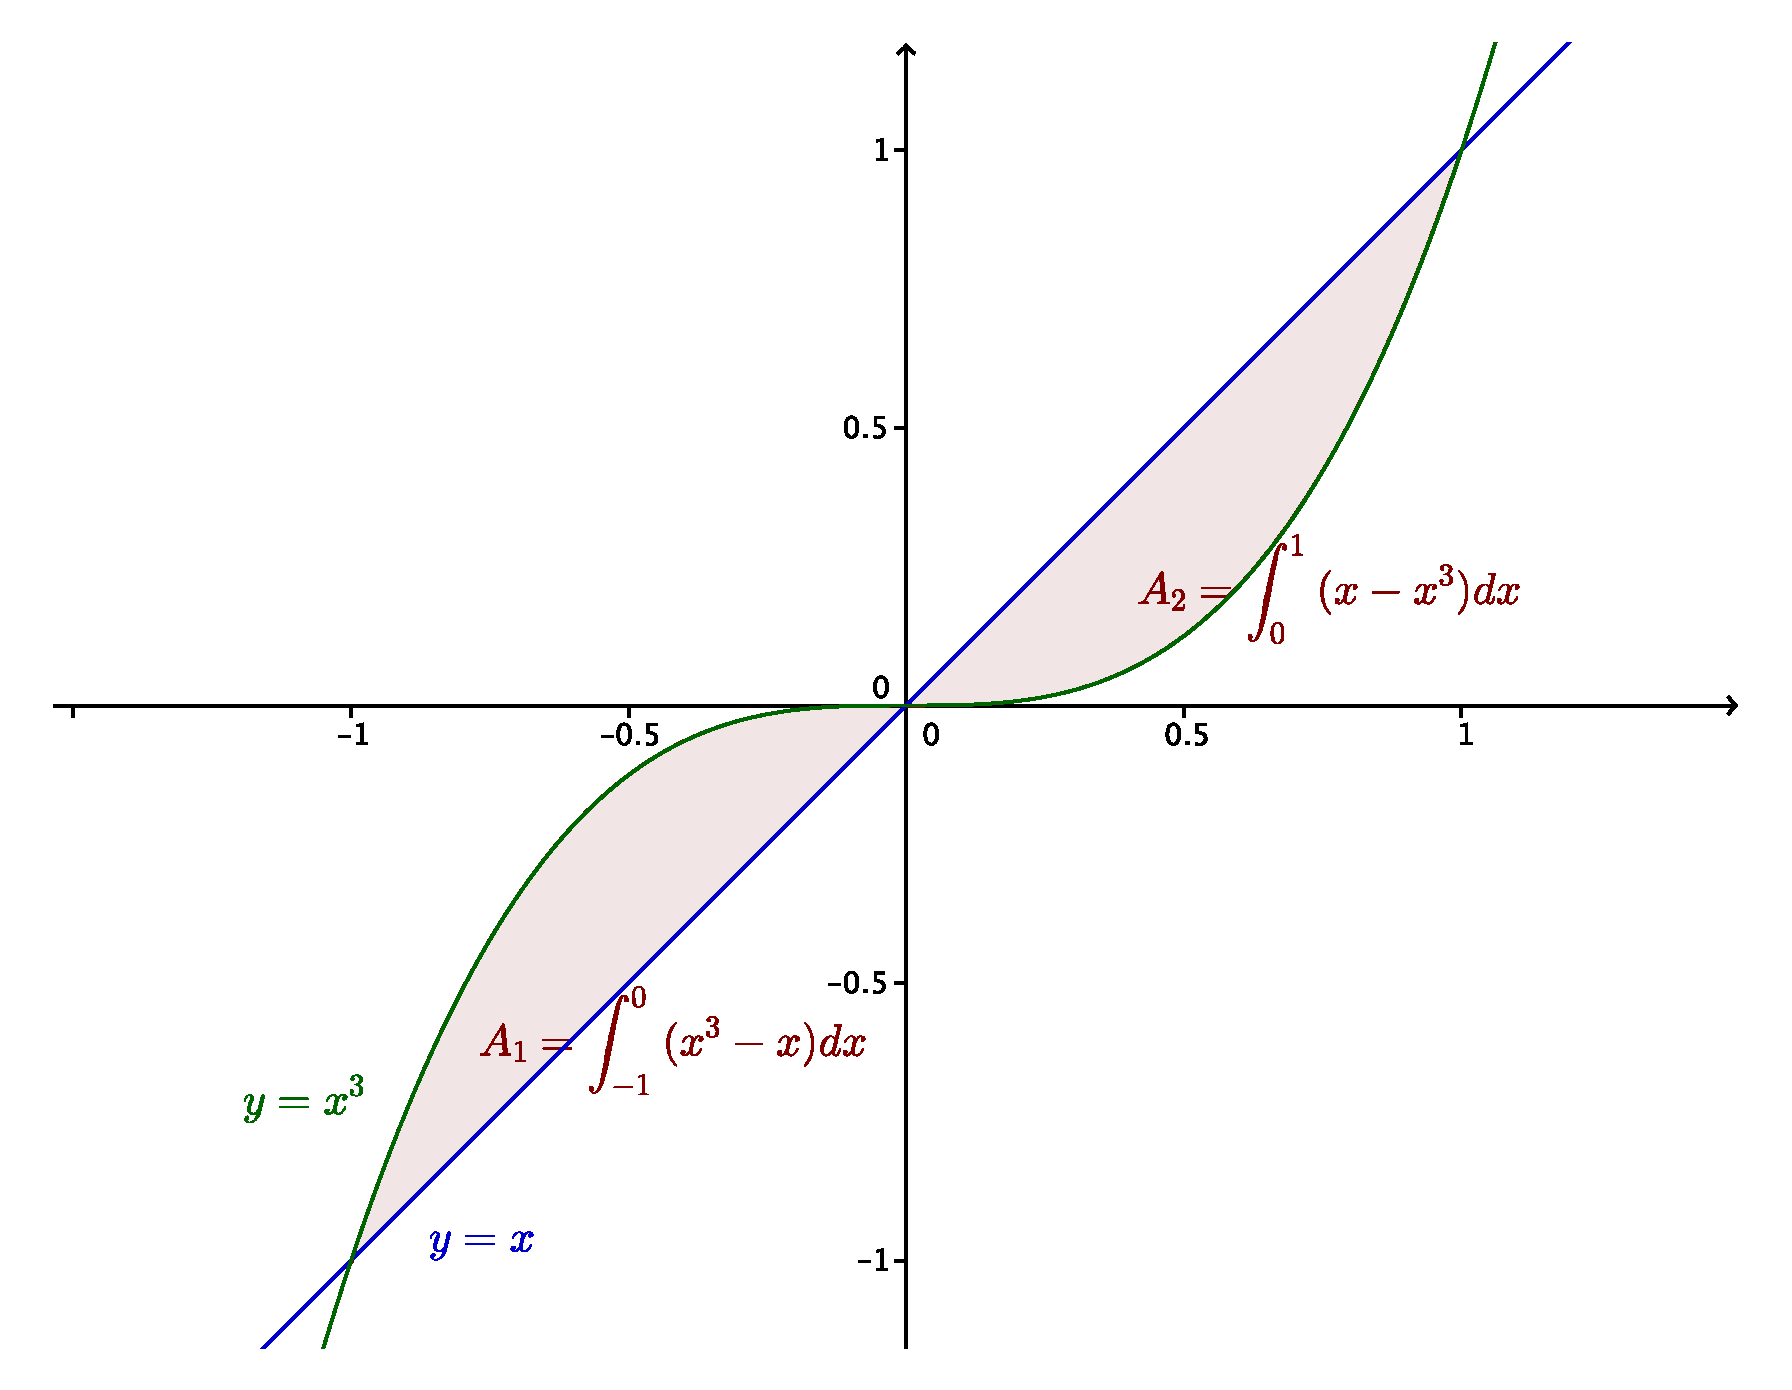
\includegraphics[width=0.8\textwidth]{WS4-1e}
\end{center}

The curves intersect if $x^3=x$, or $x^3-x = x(x-1)(x+1)=0$. There are thus two regions enclosed: the region below $y=x^3$ and above $y=x$, for $-1\leq x\leq 0$, and the region below $y=x$ and above $y=x^3$, for $0\leq x\leq 1$. By symmetry (both functions are odd), the areas of the two regions are equal. The area is therefore
\[
 A =2\int_0^1(x-x^3)\,dx = 2\left.\left(\frac{x^2}{2}-\frac{x^4}{4}\right)\right|_0^1 = \frac{1}{2}.
\]


\newpage

 \item $y=x$, $y=5x$, and $y=6-x^2$, in the first quadrant. 

\begin{center}
 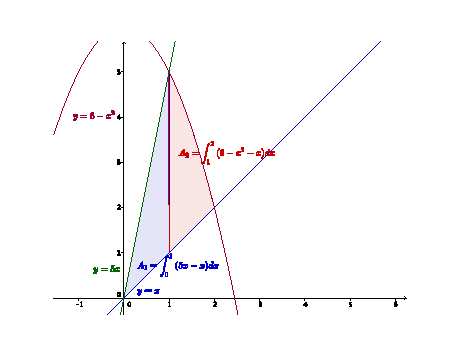
\includegraphics[width=0.8\textwidth]{WS4-1f}
\end{center}

Again we see that there are two areas to consider. The line $y=5x$ intersects the parabola $y=6-x^2$ when $6-x^2=5x$, or $x^2+5x-6 = (x+6)(x-1)=0$. The point of intersection in the first quadrant is therefore $x=1, y=5$. The line $y=x$ intersects the parabola $y=6-x^2$ when $6-x^2=x$, or $x^2+x-6=(x+3)(x-2)=0$. The point of intersection in the first quadrant is therefore $x=2, y=2$. The area is given by
\begin{align*}
 A & = \int_0^1(5x-x)\,dx + \int_1^2(6-x^2-x)\,dx\\
&=\left.2x^2\right|_0^1 + \left.\left(6x-\frac{x^3}{3}-\frac{x^2}{2}\right)\right|_1^2\\
&=\frac{25}{6}
\end{align*}

\end{enumerate}
\newpage

\item Use calculus to find the following volumes:
\begin{enumerate}
 \item Of the solid $S$ whose base is the region of the $xy$-plane bounded by $y=x^2$ and $y=2-x^2$, and whose cross-sections parallel to the $y$-axis are squares.

\begin{center}
 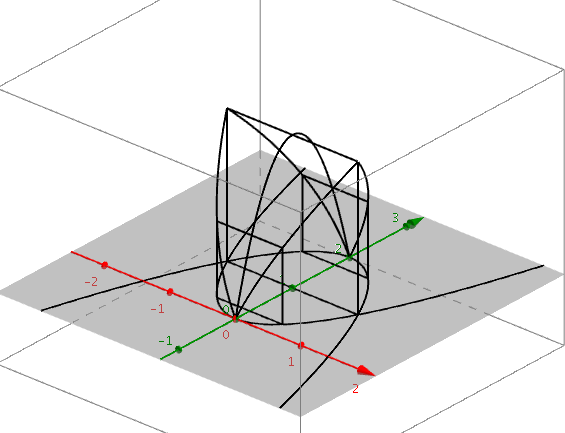
\includegraphics[width=0.6\textwidth]{WS4-2a.png}
\end{center}
The base of each square has width $y_1-y_2 = 2-x^2-x^2 = 2-2x^2$, so the cross-sectional area is $A(x) = (2-2x^2)^2 = 4-8x^2+4x^4$. The two parabolas intersect when $x=\pm 1$, so the volume is
\[
 V=\int_{-1}^1A(x)\,dx = \int_{-1}^1(4-8x^2+4x^4)\,dx = \frac{64}{15}.
\]
\newpage

 \item Of a right circular cone whose height is 12 and base radius is 4.


 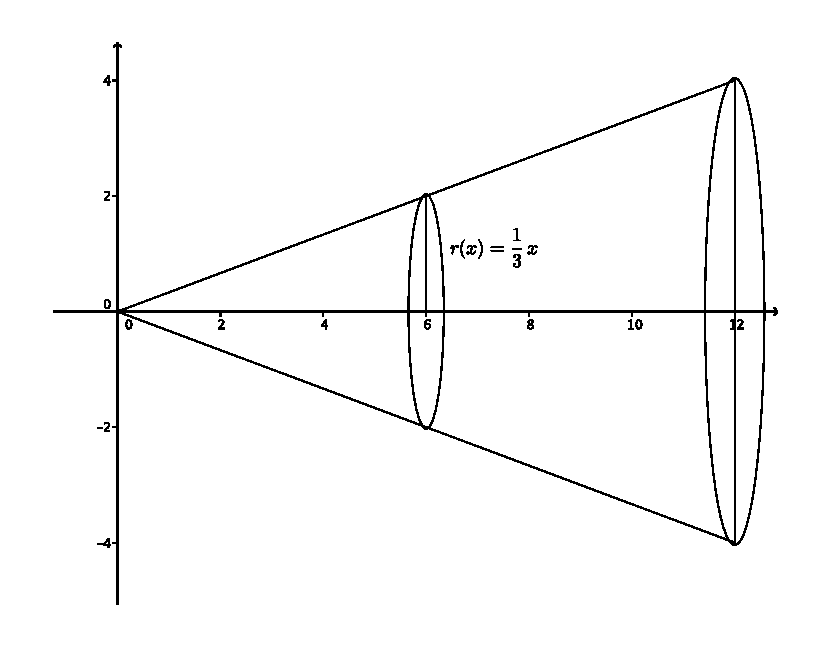
\includegraphics[width=0.75\textwidth]{WS4-2b}


To keep things simple, we orient our cone with vertex at the origin and base at $x=12$, so that the radius as a function of $x$ is given by $r(x)=\frac{1}{3}x$. (If you put the base along the $y$-axis the radius is $4-\frac{1}{3}x$ and the integral is a lot more complicated, although of course the answer works out to be the same.) Cross-sections of the cone are disks, with cross-sectional area $A(x) = \pi r(x)^2$, so the volume is
\[
 V = \int_0^{12}A(x)\,dx = \pi\int_0^{12}\frac{x^2}{9}\,dx = \left.\frac{\pi}{27}x^3\right|_0^{12} = 64\pi.
\]
\newpage

 \item The region bounded by $y=4-x^2$ and $y=0$, when rotated about
\begin{enumerate}
 \item the $x$-axis.


 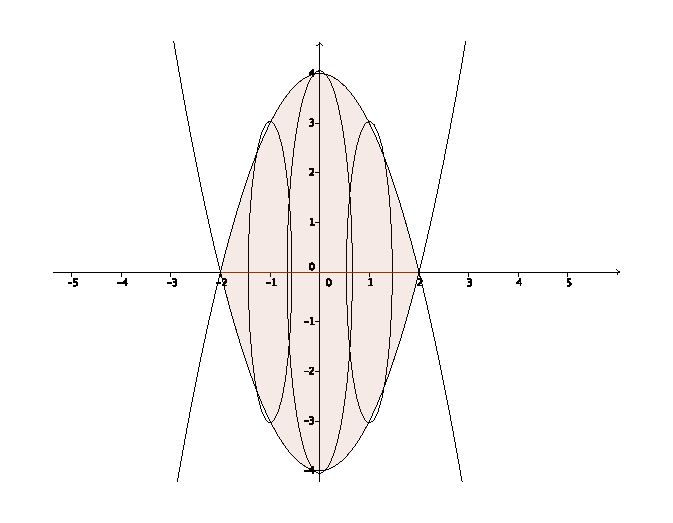
\includegraphics[width=0.75\textwidth]{WS4-2ci}


We have a solid of revolution, so cross-sections are disks, with radius $r(x)=4-x^2$. The cross-sectional area is therefore $A(x)=\pi(4-x^2)^2$, and the volume is given by
\[
 V = \int_{-2}^2A(x)\,dx = \pi\int_{-2}^2(16-8x^2+x^4)\,dx.
\]
Since the integrand is even, we have
\[
 V=2\pi\int_0^2(16-8x^2+x^4)\,dx = 2\pi\left.\left(16x-\frac{8}{3}x^3+\frac{1}{5}x^5\right)\right|_0^2 = \frac{512\pi}{15}.
\]
\newpage

 \item the line $y=-1$.


 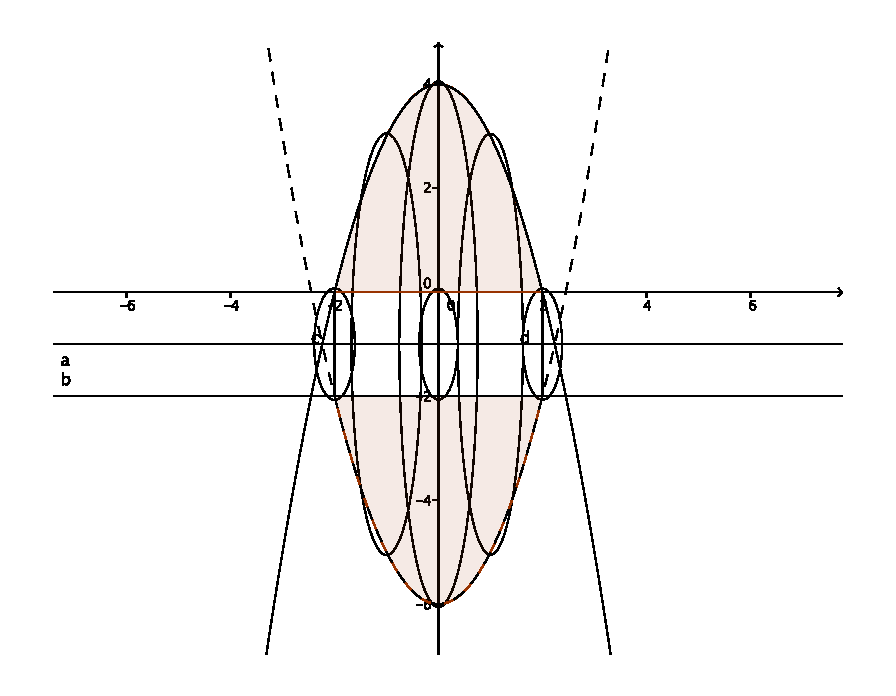
\includegraphics[width=0.75\textwidth]{WS4-2cii}


We have a solid of revolution, but since the axis of rotation is one unit away from the bottom of the region being revolved about the axis, cross-sections are washers. The inner radius is 1, and the outer radius is $r(x)=y(x)+1=5-x^2$, so the cross-sectional area is
\[
 A(x) = \pi r_{out}(x)^2-\pi r_{in}(x)^2 = \pi(5-x^2)^2-\pi(1)^2 = 24-10x^2+x^4.
\]
Noting that $A(x)$ is an even function, we have
\[
 V = \int_{-2}^2A(x)\,dx = 2\int_0^2(24-10x^2+x^4)\,dx = \pi\left.\left(24x-\frac{10}{3}x^3+\frac{1}{5}x^5\right)\right|_0^2 = 16\pi\left(\frac{26}{15}\right).
\]
\newpage

 \item the line $x=2$.


 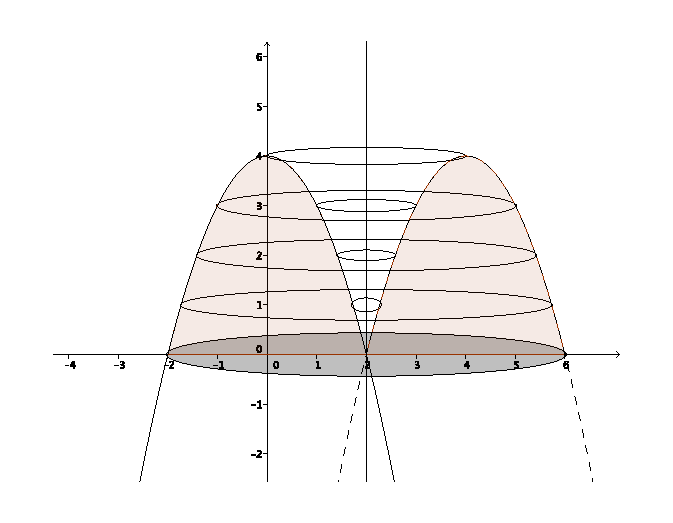
\includegraphics[width=0.75\textwidth]{WS4-2ciii}


This time we're revolving about an axis parallel to the $x$-axis, so we have to solve for $x$ in terms of $y$. We find $x=\pm \sqrt{4-y}$, where the positive root corresponds to the right half of the parabola, and the negative root to the left half. The cross-sections are again washers if we slice horizontally. The inside of the washer corresponds to the right of the parabola, and the outside of the washer corresponds to the left of the parabola, so the inner and outer radii of the washer are given by
\[
 r_{in}(y) = 2-x = 2-\sqrt{4-y} \quad \text{ and } \quad r_{out}(y) = 2-(-\sqrt{4-y}) = 2+\sqrt{4-y}.
\]
The cross-sectional area is therefore
\[
 A(y) = \pi r_{out}(y)^2-\pi r_{in}(y)^2 = \pi (2+\sqrt{4-y})^2 - \pi (2-\sqrt{4-y})^2 = 8\pi\sqrt{4-y},
\]
so the volume is given by
\[
 V = \int_0^4 A(y)\,dy = 8\pi\int_0^4 (4-y)^{1/2}\,dy = \left.-\frac{16\pi}{2}(4-y)^{3/2}\right|_0^4 = \frac{128\pi}{3}.
\]

\end{enumerate}
\newpage

 \item The region bounded by the curves $y^2=x$ and $x=2y$, when revolved around the $y$-axis.


 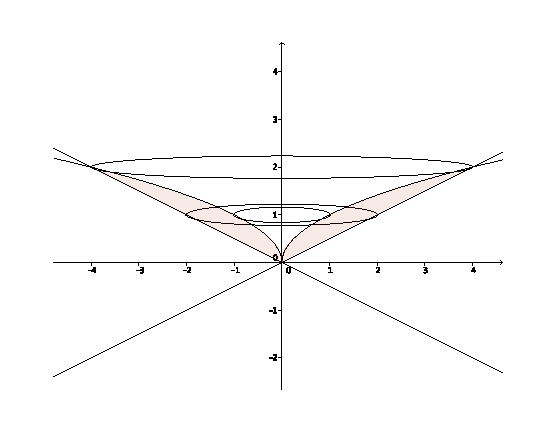
\includegraphics[width=0.8\textwidth]{WS4-2d}


From the diagram above we see that we have a solid whose cross-sections parallel to the $x$-axis are washers, with inner radius $r_{in}(y)=y^2$, and outer radius $r_{out}(y)=2y$, with $0\leq y\leq 2$. The cross-sectional area is
\[
 A(y) = \pi r_{out}(y)^2-\pi r_{in}(y)^2 = \pi (4y^2-y^4).
\]
The volume is therefore
\[
 V = \int_0^2A(y)\,dy = \pi \int_0^2 (4y^2-y^4)\,dy = \pi\left.\left(\frac{4}{3}y^3-\frac{1}{5}y^5\right)\right|_0^2 = \frac{64\pi}{15}.
\]


\end{enumerate}

\end{enumerate}


\end{document}